% https://tex.stackexchange.com/a/749595/322482
\documentclass[tikz,border=1cm]{standalone}
\usetikzlibrary{positioning}    % not needed for matrix approach
\usetikzlibrary{matrix,fit}     % for matrix part
\begin{document}
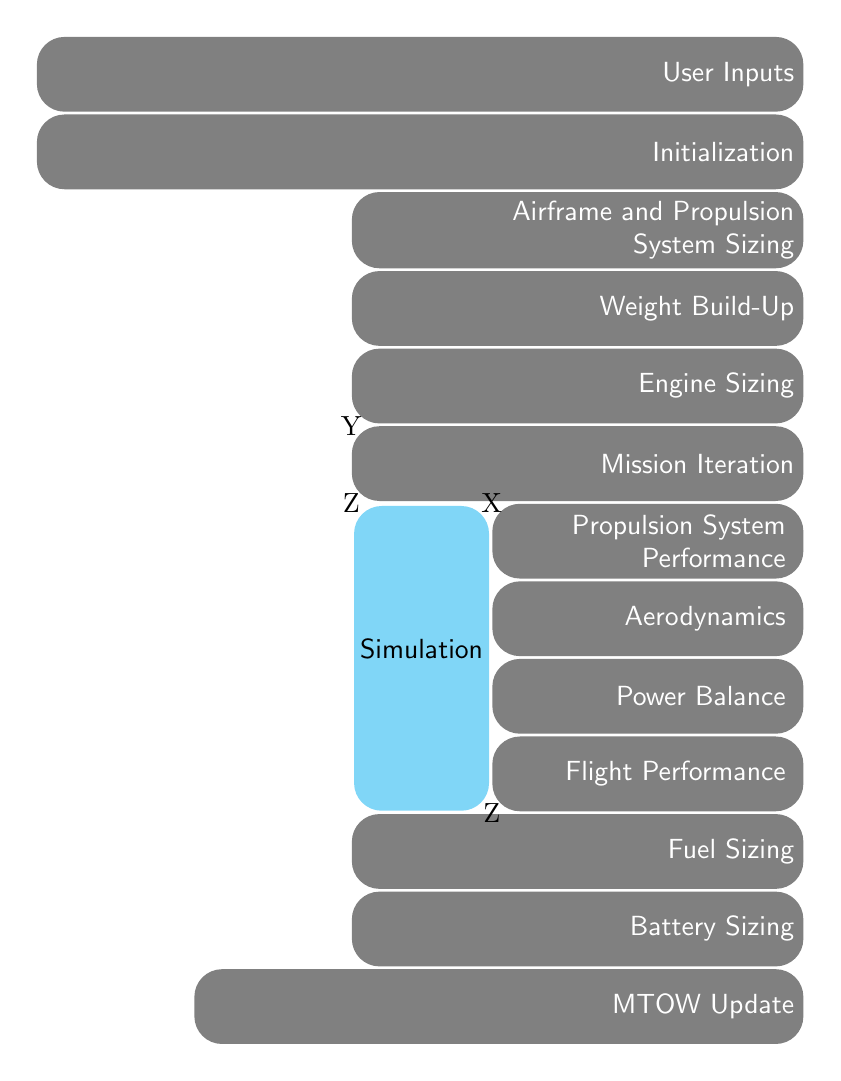
\begin{tikzpicture}[
    ga/.style={
        anchor=east,
        fill=gray,
        align=right,
        text width=3.5cm,
        text=white,
        font=\sffamily,
        minimum width=3.95cm,
        minimum height=.95cm,
        rounded corners=10pt,
    },
    gb/.style={ga,text width=5.5cm,},
    gc/.style={ga,text width=7.5cm,},
    gd/.style={ga,text width=9.5cm,},
    bl/.style={
        fill=cyan!50,
        align=center,
        font=\sffamily,%\large,
        rounded corners=10pt,
        inner sep=-1pt,
    },
]
    \matrix (m) [matrix of nodes, row sep=1pt]{
        |[gd]|User Inputs \\ 
        |[gd]|Initialization\\     
            |[gb]|  Airframe and Propulsion\par System Sizing\\
            |[gb]|  Weight Build-Up \\            
            |[gb]|  Engine Sizing  \\            
            |[gb]|  Mission Iteration \\           
              |[ga]|    Propulsion System\par Performance  \\   
              |[ga]|    Aerodynamics \\                     
              |[ga]|    Power Balance\\                    
              |[ga]|    Flight Performance \\          
            |[gb]|  Fuel Sizing \\                  
            |[gb]|  Battery Sizing \\                  
          |[gc]| MTOW Update\\                        
    };
    % ~~~ demo: identifying coordinates ~~~~~~~~~~~~
    \node at (m-7-1.north west) {X};
    \node at (m-6-1.north west) {Y};
    \node at (m-6-1.north west |- m-7-1.north west) {Z};
    \node at (m-10-1.north west |- m-11-1.north west) {Z};
    % ~~~ final fit via perpendicular coordinates ~~~~~~~~~
    \node[bl,fit=(m-6-1.north west  |- m-7-1.north west) 
                 (m-10-1.north west |- m-11-1.north west)]{Simulation};
\end{tikzpicture}

% ~~~~~~~~~~~~~~~~~~~~~~~~~~~~~~~~~~~~~~~~~~~~~~~
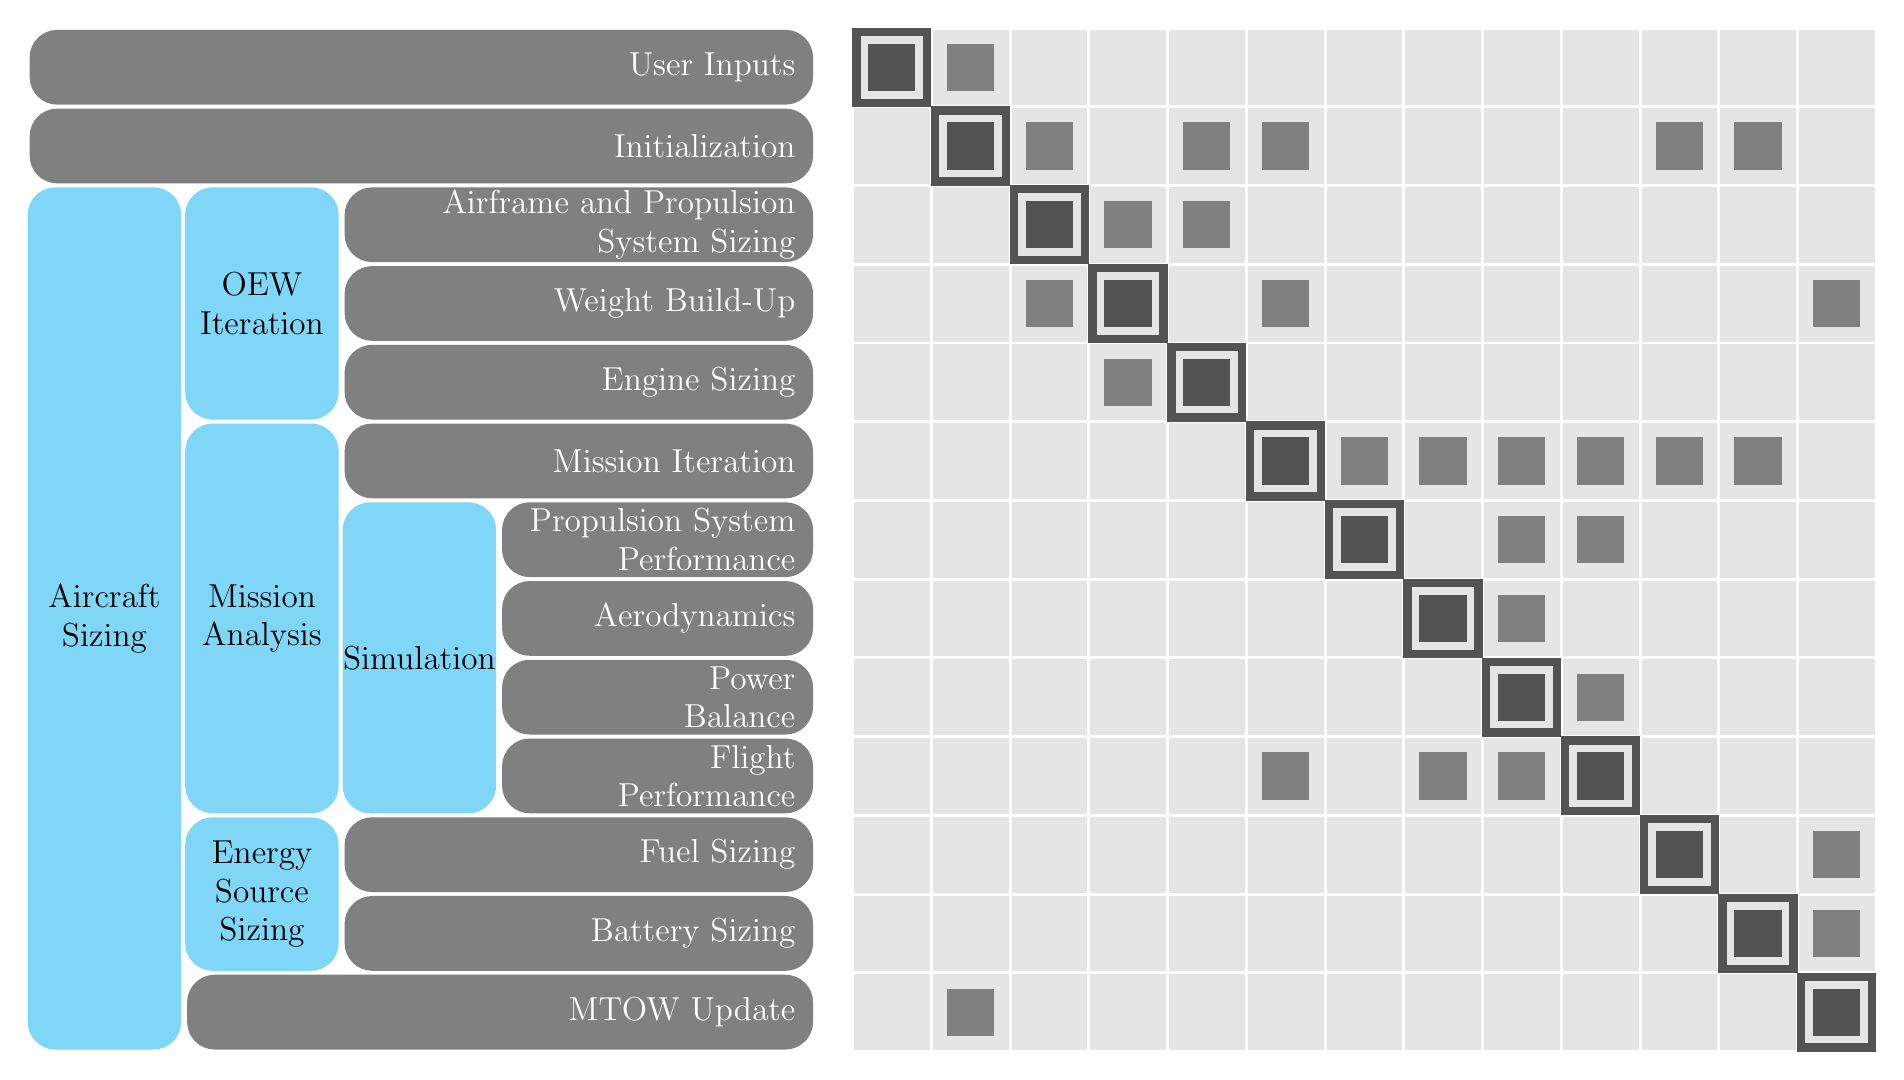
\begin{tikzpicture}[
    on grid,
    every node/.style={
        inner sep=0pt,
        outer sep=0pt,
    },
    outer/.style={
        draw=gray!65!black,rectangle,
        line width=3pt,
        minimum size=.9cm,
    },
    inner/.style={
        fill=#1,rectangle,
        line width=3pt,
        minimum size=.6cm,
    },
    background/.style={
        draw=white,
        line width=.25pt,
        rectangle,
        minimum size=.975cm,
        fill=gray!20,
    },
    leftnodea/.style n args={2}{
        fill=cyan!50,
        align=center,
        font=\large,
        minimum width=#1 cm-.05cm,
        minimum height=#2 cm-.05cm,
        rounded corners=10pt,
    },
    leftnodeb/.style n args={2}{
        fill=gray,
        align=right,
        text width=#1cm -.5cm,% 
        text=white,
        font=\large,
        minimum width=#1 cm-.05cm,
        minimum height=#2 cm-.05cm,
        rounded corners=10pt,
    },
]
    % ~~~ refactored ~~~~~~~~~~~~~~~~~~~~~~~~~~~~~~~~~~~~~~~~~~~~~~
    \newcommand\ga[2]{\node[leftnodeb={ 4}{1},anchor=east] at (#1) {#2}}
    \newcommand\gb[2]{\node[leftnodeb={ 6}{1},anchor=east] at (#1) {#2}}
    \newcommand\gc[2]{\node[leftnodeb={ 8}{1},anchor=east] at (#1) {#2}}
    \newcommand\gd[2]{\node[leftnodeb={10}{1},anchor=east] at (#1) {#2}}
    
    \foreach \x in {0,...,12}{
        \foreach \y in {0,...,12}{
            \node[background] at (\x,\y) {};
        }
    }
    \foreach \x [evaluate=\x as \y using 12-\x] in {0,...,12}
    {
        \node[outer]                at (\x,\y) {};
        \node[inner=gray!65!black]  at (\x,\y) {};
    }
    \foreach \x/\y in {%
        1/12,
        2/11,4/11,5/11,10/11,11/11,
        3/10,4/10,
        2/9,5/9,12/9,
        3/8,
        6/7,7/7,8/7,9/7,10/7,11/7,
        8/6,9/6,
        8/5,
        9/4,
        5/3,7/3,8/3,
        12/2,
        12/1,
        1/0%no comma after
    }{
        \node[inner=gray] at (\x,\y) {};
    }
    % ~~~ first part refactored -> redundancy via anchor=east ~~~~~~~~~~
    \begin{scope}[xshift=-1cm]
    \gc{0,0}{MTOW Update};
    \gb{0,1}{Battery Sizing};
    \gb{0,2}{Fuel Sizing};
    \ga{0,3}{Flight\\Performance};
    \ga{0,4}{Power\\Balance};
    \ga{0,5}{Aerodynamics};
    \ga{0,6}{Propulsion System\\Performance};
    \gb{0,7}{Mission Iteration};
    \gb{0,8}{Engine Sizing};
    \gb{0,9}{Weight Build-Up};
    \gb{0,10}{Airframe and Propulsion\\System Sizing};
    \gd{0,11}{Initialization};
    \gd{0,12}{User Inputs};
    
    % ~~~ can be treated separately ~~~~~~~~
    \node[leftnodea={2}{11}] at (-9,5) {Aircraft\\Sizing};
    \node[leftnodea={2}{2}] at (-7,1.5) {Energy\\Source\\Sizing};
    \node[leftnodea={2}{5}] at (-7,5) {Mission\\Analysis};
    \node[leftnodea={2}{3}] at (-7,9) {OEW\\Iteration};
    \node[leftnodea={2}{4}] at (-5,4.5) {Simulation};
    \end{scope}
\end{tikzpicture}

\end{document}